\section{Technical Discussion and R\&D Plan}
\label{sec:research}

This section will first describe background information on both BECS
conroller equipment and the general state-of-the-art in differential
privacy.  Following that is the description of the research to be
performed.  We finish with a research plan, timeline, and a short
description of the research items deferred to Phase II.

\subsection{Background}
\label{sec:background}

\subsubsection{IoT Data Collected by BECS Technology}

BECS Technology's controllers are fairly typical devices
in the Internet of Things (IoT).
The controller itself monitors various aspects of water chemistry:
pH, oxidation-reduction potential (ORP), free chlorine concentration,
temperature, conductivity, turbidity, etc. 
Based on these readings, the controller takes various actions
(feeding chemical, adjusting recirculation flow rate, etc.) to maintain
the water chemistry within desired parameters.
Alarm conditions trigger notifications to service personnel.
Sensor values and actions are all logged internally,
and these logs are frequently used when diagnosing the causes
of alarms or other anomalous events.
Remote access to all of the above information is
clearly to the benefit of the equipment owners/operators.

While the notion of IoT might be new,
the fundamental capability to access controller information remotely
is not.  BECS Technology's controllers have supported remote communications
for more than 2 decades.
Early controllers used modems attached to the telephone network, today
controllers support TCP/IP connectivity via the Internet.

Remote capabilities include viewing of current status, downloading
of data logs, and configuration of the controller.
Figure~\ref{console} illustrates a realtime view of water chemistry
for a specific body of water
as remotely displayed on a PC screen.  Four readings are being shown:
pH (at\,7.1), ORP (at 750\,mV), temperature (at 83\,\degree F), and
free chlorine (at 1.0\,ppm).  Also indicated are the set points and
high and low alarm points for each reading as well as the control
outputs (in this example control is based on pH and ORP).
The two dials at the bottom show a pair of indices
(Langelier Saturation Index and Ryznar Stability Index)
which are indicators of the scaling properties of the water~\cite{mb88}.
The panel on the left allows the user to navigate to different
controllers (either at the same or a different physical location).
The tabs at the top allow the user to access a menu tree that
can examine and/or modify a multitude of parameters on the controller.

\begin{figure}[t]
 \center
\includegraphics[width=0.8\columnwidth]{console}
    \caption{Console display of controller at remote location.}
    \label{console}
\end{figure}

Figure~\ref{graph} illustrates data logs collected over a 2 day period.
The same four readings are plotted on the top graph, and the bottom
graph gives indications of control actions, alarms, and other events.
In the top curve, one can readily see disturbances in the pH at noon
on both days.
The additional window on the right shows the instantaneous values
at the position of the cursor (the vertical line positioned
by the user at 9am on the first day).
As above, the leftmost panel supports navigation to different
controllers.

\begin{figure}[t]
 \center
\includegraphics[width=0.9\columnwidth]{graph}
    \caption{Plot of controller data logs.}
    \label{graph}
\end{figure}

To reinforce the notion that remote communications capability is
nothing new, the data logs shown are from a time period more than a
decade ago (in 2006).
While the two figures show images from a desktop PC screen, modern
remote communications capability is also supported via apps that
run on smartphones and tablets.

In addition to diagnosing the root causes of errors in the water
chemistry, the historical logs also enable the tracking of
parameter changes by operators as well as support the demonstration
and documentation of regulatory compliance.
Using EZAnalytics\texttrademark{}~\cite{ccgss17}, these data logs
are collected automatically and the information retained in the
cloud for easy access by the owners/operators of the equipment.

The security of these controllers is
state-of-the-art~\cite{ccgss16,ccgss18}, with special attention given
to ease-of-use considerations, as there is ample evidence that
security measures that are difficult to implement are frequently
circumvented by users~\cite{gefen2000relative,hertzum2004usable,schneier16}.

Currently, the data access model is such that equipment owners have
access to data from their own controllers, but there is no data sharing.
Because individual owners each typically have a limited number of
control systems (between 1 and 10 controllers would be typical at an
individual facility), there is limited data available for
learning to take place.  This is true whether the learning is
happening in an automated way (e.g., using modern
machine learning techniques) or manually (using visualization tools).
Each of these approaches will benefit from broader experiential coverage.
Changing this current state of affairs is the specific purpose of the
proposed research project.

\subsubsection{Privacy Theory}

Our goal is to make aggregated data available while preserving the
privacy of individual data owners.  Differential privacy
provides strong theoretical guarantees in this area.  Dwork and
Roth~\cite{dwork11,dr14} provided the seminal initial work in this
area, and more recently Nguyen et al.~\cite{nkk13} and
Wang et al.~\cite{wll15} have reviewed the differential
privacy literature as it has been applied to various practical circumstances.
A number of groups have contributed to differentially private hierarchical data
(referred to as histograms)~\cite{hrms10,xxy10}.
Most relevant to our interest is the work of
Rastogi and Nath~\cite{rn10} and
Fan and Xiong~\cite{fx12,fx14}, who describe approaches to time series data.

Recently, Uber has released an open source project that supports
SQL queries~\cite{uber2,Near18,uber}.  This project is based in part
on work by Johnson et al.~\cite{jns18}, called elastic sensitivity, and
also supports several additional differential privacy mechanisms.
While it does not directly target time series data,
and it certaintly has not quantitatively assessed the tradeoffs between
privacy budget and utility in a water chemistry context, it does
point to an effective approach for deploying differential privacy
in the field.  We will leverage this open source release in our
development efforts, which will enable us to focus more on the questions
of ``how well does this work?'' rather than ``how do we get it to work.''

Differential privacy is far from the only approach to the problem.
Others have described $k$-anonymity~\cite{samarati01,sweeney02},
$l$-diversity~\cite{mkgv07},
other techniques aimed at hierarchical data sets~\cite{lnpr14}, and some
have asserted that multiple, combined approaches are superior to any
individual technique~\cite{ct13}.
TIPPERS~\cite{tippers} is an experimental infrastructure, built on a
Honeywell building management system, that supports privacy research
in the IoT space.

The core notion of differential privacy, informally stated, is that whether
or not a single individual chooses to share his/her data to be a part of
the collected data set does not impact the conclusions one draws from
the data set.
This is typically accomplished by perturbing the results of queries
against the data set by some random amount.
Moving towards more formality~\cite{dr14}, a randomized algorithm $\mathcal{M}$
is $(\epsilon,\delta)$-\emph{differentially private} if for all
$\mathcal{S} \subseteq \mbox{Range}(\mathcal{M})$ and datasets $x$ and $y$
differing in at most one record:
\begin{equation}
\Pr[\mathcal{M}(x) \in \mathcal{S}] \leq e^\epsilon \cdot \Pr[\mathcal{M}(y)
\in \mathcal{S}] + \delta
\label{eqn:dp}
\end{equation}
where the probability is over the randomness of the algorithm $\mathcal{M}$.
The parameter $\epsilon$ is often called the
\emph{privacy budget}~\cite{McSherry09}; $(\epsilon,\delta)$-differential
privacy ensures that for all adjacent $x$ and $y$, the privacy loss
(as defined in~\cite{dr14}) will
be bounded by $\epsilon$ with probability at least $1-\delta$.
Operationally, it is possible to achieve differential privacy by adding
i.i.d.~noise to query results.

Our circumstance is one in which time series data is to be queried, and we
wish to preserve the privacy of the data owners (rather than that of
an individual record).
Fan and Xiong~\cite{fx12,fx14} describe a mechanism in which the time
series are first sampled, perturbed (by adding i.i.d.~noise), and then
the released series is composed using prediction (for the non-sampled
points) and prediction-correction (for the sampled points).  It is this
approach that we will initially explore.

\subsection{Research}

The goal of the overall system is to support exploration of aggregated data. 
To achieve this goal, we will leverage our current IoT infrastructure
to implement privacy-preserving data aggregation techniques from the
differential privacy literature.
The data processing, computation, and aggregation occur in the
back-end where the data reside.
The processed data sent to the front-end visualization system will
contain aggregated data for clients and stakeholders to interact with.

During Phase~I, our focus will be on addressing the following two
research questions.
\begin{enumerate}
\item[\textbf{R1:}] Can we effectively reduce differential privacy theory to practice,
balancing the conflicting concerns of privacy budget and data utility, in
the context of water chemistry control?
\item[\textbf{R2:}] Can we effectively communicate aggregated time series data,
with the inherent uncertainty imposed by differential privacy, to end users?
\end{enumerate}

We anticipate addressing the first question through empirical evaluation,
exercising one (or more) privacy-preservation algorithms across water
chemistry IoT data and assessing the resulting output in the privacy
versus utility tradeoff space.  We will address the second question by
exploring several visualization approaches and assessing their effectiveness
through user studies.\footnote{For all user studies, we will seek the
appropriate human subjects approvals through the IRB at Washington
Univ.~in St.~Louis.}

\subsubsection{R1: Data Aggregation and Privacy Preservation}

We are interested in assessing our ability to reduce differential
privacy theory into effective practice, and our approach to achieving
that goal is empirical evaluation.  That implies collecting data,
performing experiments, and evaluating the experimental outcomes.
We will describe each of these in turn.

\paragraph{Data Sources}
The EZAnalytics\texttrademark{} system currently provides cloud-based access to
water chemistry data owned by the individual user.
BECS is the trusted curator of that data, responsible for its security,
integrity, and availability.  To provide experimental
data for the proposed privacy preservation research, we will query 
current customers and ask permission to use historical data from their
sites.  There are a number of customers that regularly assist
us in evaluating new products, etc., at their site, such that we anticipate
no difficulty in achieving data access from real-world installations.

In addition to customer data, BECS maintains a wet wall test facility in
its plant (see Facilities, Equipment and Other Resources) that has multiple
instances of water treatment control and monitoring equipment installed.
Data are available from this facility going back several years.

\paragraph{Experiments}
Our initial empirical investigation will focus on the approaches
described by Fan and Xiong~\cite{fx12,fx14}, utilizing their
FAST (Filtering and Adaptive Sampling for differentially private
Time-series monitoring) framework. Individual experiments will have
as inputs:
\begin{itemize}
\item an example aggregated time series data set,
\item settings for the privacy budget
(i.e., values of $\epsilon$ and $\delta$),
\item parameter values for FAST (i.e., see Table~1 of \cite{fx14}), and
\item prediction/correction filter for FAST (Kalman vs.~Monte Carlo)
\end{itemize}
and will provide an output time series that is differentially private.
Using any number of techniques (e.g., relative error, correlation analysis), 
we can then compare the input (non-private) time series to the output
time series.
We will use $2^k$ factorial experimental design~\cite{Jain91}
to reduce the overall empirical search space to manageable levels,
adding experiments as needed to fill in portions of the space that
appear interesting.

Of course, the real world is never as simple as implied by the previous
paragraph.  E.g., $\delta= 0$ in the published version of FAST.
Next, we describe our approach to several of the
complications that we must plan to address.
In the time series formulation of Fan and Xiong, they only consider
a single series, while in our case we have multiple series measurements
from a single body of water.  A typical system will monitor pH,
free chlorine concentration, oxidation-reduction potential (ORP),
and temperature.
Optional additional measurements might include recirculation rate, water level,
feed chemical inventory stocks, and many others.
As such,
the sensitivity of each aggregate query needs to be analyzed
for each measure in order to hide the contribution of each client.

It would be completely unreasonable to consider these separate measurements
to be independent.  In fact, there is ample reason to believe they are
strongly correlated.  For example, chlorine control is, in many cases,
driven from an ORP reading rather than a free chlorine reading.
As such, we will need to extend the approach of Fan and Xiong to support
multiple time series.
We will start by using the same reasoning as Fan and Xiong.  For $n$
series, we will allocate $\epsilon / n$ of the privacy budget to each series.

If this initial approach is too constraining, we will explore alternative
partitionings of the privacy budget, in particular, approaches that dynamically
form the partitioning guided by the tradeoffs between privacy budget
and utility (which are likely to be different for different sensor signals).

While our initial focus will be on the techniques described by Fan and Xiong,
an alternative approach to time series data is presented by Rastogi
and Nath~\cite{rn10}.  In their approach, the time domain data are
transformed into the frequency domain, appropriate additive noise
is inserted to ensure differential privacy, and the inverse transform
returns the data to the time domain.
This technique requires that the entire data set be available prior to
release; however, that is not an insurmountable obstacle in our
circumstance.

Another practical consideration that we much address is the fact that, in
addition to traditional time series data, our data sets also include
event data (e.g., alarm conditions, chemical feed, control parameter
changes).  For those that can be effectively encoded as binary variables
(e.g., alarm status, chemical feed), we will start with that encoding.
One possibility for discrete events is to encode their inter-event time
and ensure that it is differentially private.
Another is to use the $w$-event privacy notions introduced by
Kellaris et al.~\cite{Kellaris14}.
In the most pessimistic case, we might need to suppress some raw data,
if we cannot ensure its disclosure maintains privacy.  In such a situation,
we clearly need to quantitatively assess the utility implications
of this choice.

To this point in the discussion, we have maintained strict compliance
with differential privacy, looking to discover whether or not we can
achieve sufficient utility at an acceptable privacy budget.  If this is
the case, we have succeeded in our goal.  If this is not the case, all
is not lost.

Clifton and Tassa~\cite{ct13} argue that other privacy preserving
mechanisms, while not as strong as differential privacy from a
theoretical perspective, are still quite valuable in practice.
Just as we cannot prove perfect security, and therefore rely on multiple
tiers of security apparatus, we can also exploit a similar approach
to data privacy.  
We will investigate a multi-tiered approach to data
privacy that has differential privacy at its core, but leverages the
additional concepts of \emph{suppression} and \emph{generalization}
which are commonly used means to transform data to comply with
$k$-anonymity and/or $l$-diversity criteria~\cite{mkgv07}.
%, as its baseline, differential privacy.  
Specifically, in our setting suppression would entail removing time
series contributions from a (small) subset of organizations, whereas
generalization would determine the level of discretization of time in
the time series.
We will use these techniques to preprocess the dataset
before applying the algorithms for making the resulting data
differentially private.
The key intuition for this approach is that suppression would serve to
reduce global sensitivity of the queries by removing organizations that are
particularly identifiable in the dataset (e.g., those which are highly
unusual).
Similarly, using coarser time series data would reduce the amount of
noise necessary to make it differentially private, at the cost of utility loss
of removing fine-grained information.
We conjecture that the combined approaches provide us with sufficient
leverage to allow for optimal balancing between utility and privacy.

%However,
%the privacy budget will be set so as to ensure utility of the released
%data.  This data will then undergo additional anonymization, such as
%$k$-anonymity~\cite{samarati01,sweeney02}
%and/or $l$-diversity~\cite{mkgv07} so as to further
%obfuscate the individual data owner's identity.
%Clearly, this will complicate the quantitative evaluation of the
%privacy versus utility tradeoff. In this case, we will evaluate what we
%can.  At the very least, since we will have access to ground truth in
%the data, a quantitative evaluation of utility will still be possible.

\paragraph{Evaluating Outcomes}
For most of our experimental results, the outcomes of an experiment
will be in the form of a multi-dimensional ROC curve
(more precisely, a multi-dimensional
regression ROC curve~\cite{Fawcett06,HO13,Mossman99}), illustrating
the tradeoffs between privacy budget (shown on one axis) and uncertainty
(shown on the other axis). If we can effectively fix the parameter $\delta$,
as has been suggested~\cite{dr14}, that leaves $\epsilon$ as the
sole parameter describing privacy budget (at least in the case where
we are only using differential privacy as the privacy mechanism), so we
are down to one dimension there.

Similarly, if we can distill the uncertainty to a summary statistic
(e.g., rms error, or some other norm), uncertainty can also be reduced
to a single dimension, and now we can actually plot a traditional ROC
curve, showing the tradeoff between privacy budget and uncertainty.
Clearly, this distillation down to a traditional ROC curve won't happen
for every case, but we will exploit it whenever we can.

Given the existence of an ROC curve that realistically communicates the
tradeoffs implied, what still remains is the judgment as to whether or
not any achievable points in the tradeoff space are acceptable (i.e.,
effectively meet the needs of end users).  Understanding
this is key to commercial
feasibility. We will evaluate this by
asking attendees at the annual sales meeting to give us feedback on 
the tradeoffs.

\subsubsection{R2: Client Visualization}

\begin{figure*}[t!]
	\centering
	\begin{subfigure}[t]{.3\columnwidth}
		\centering
		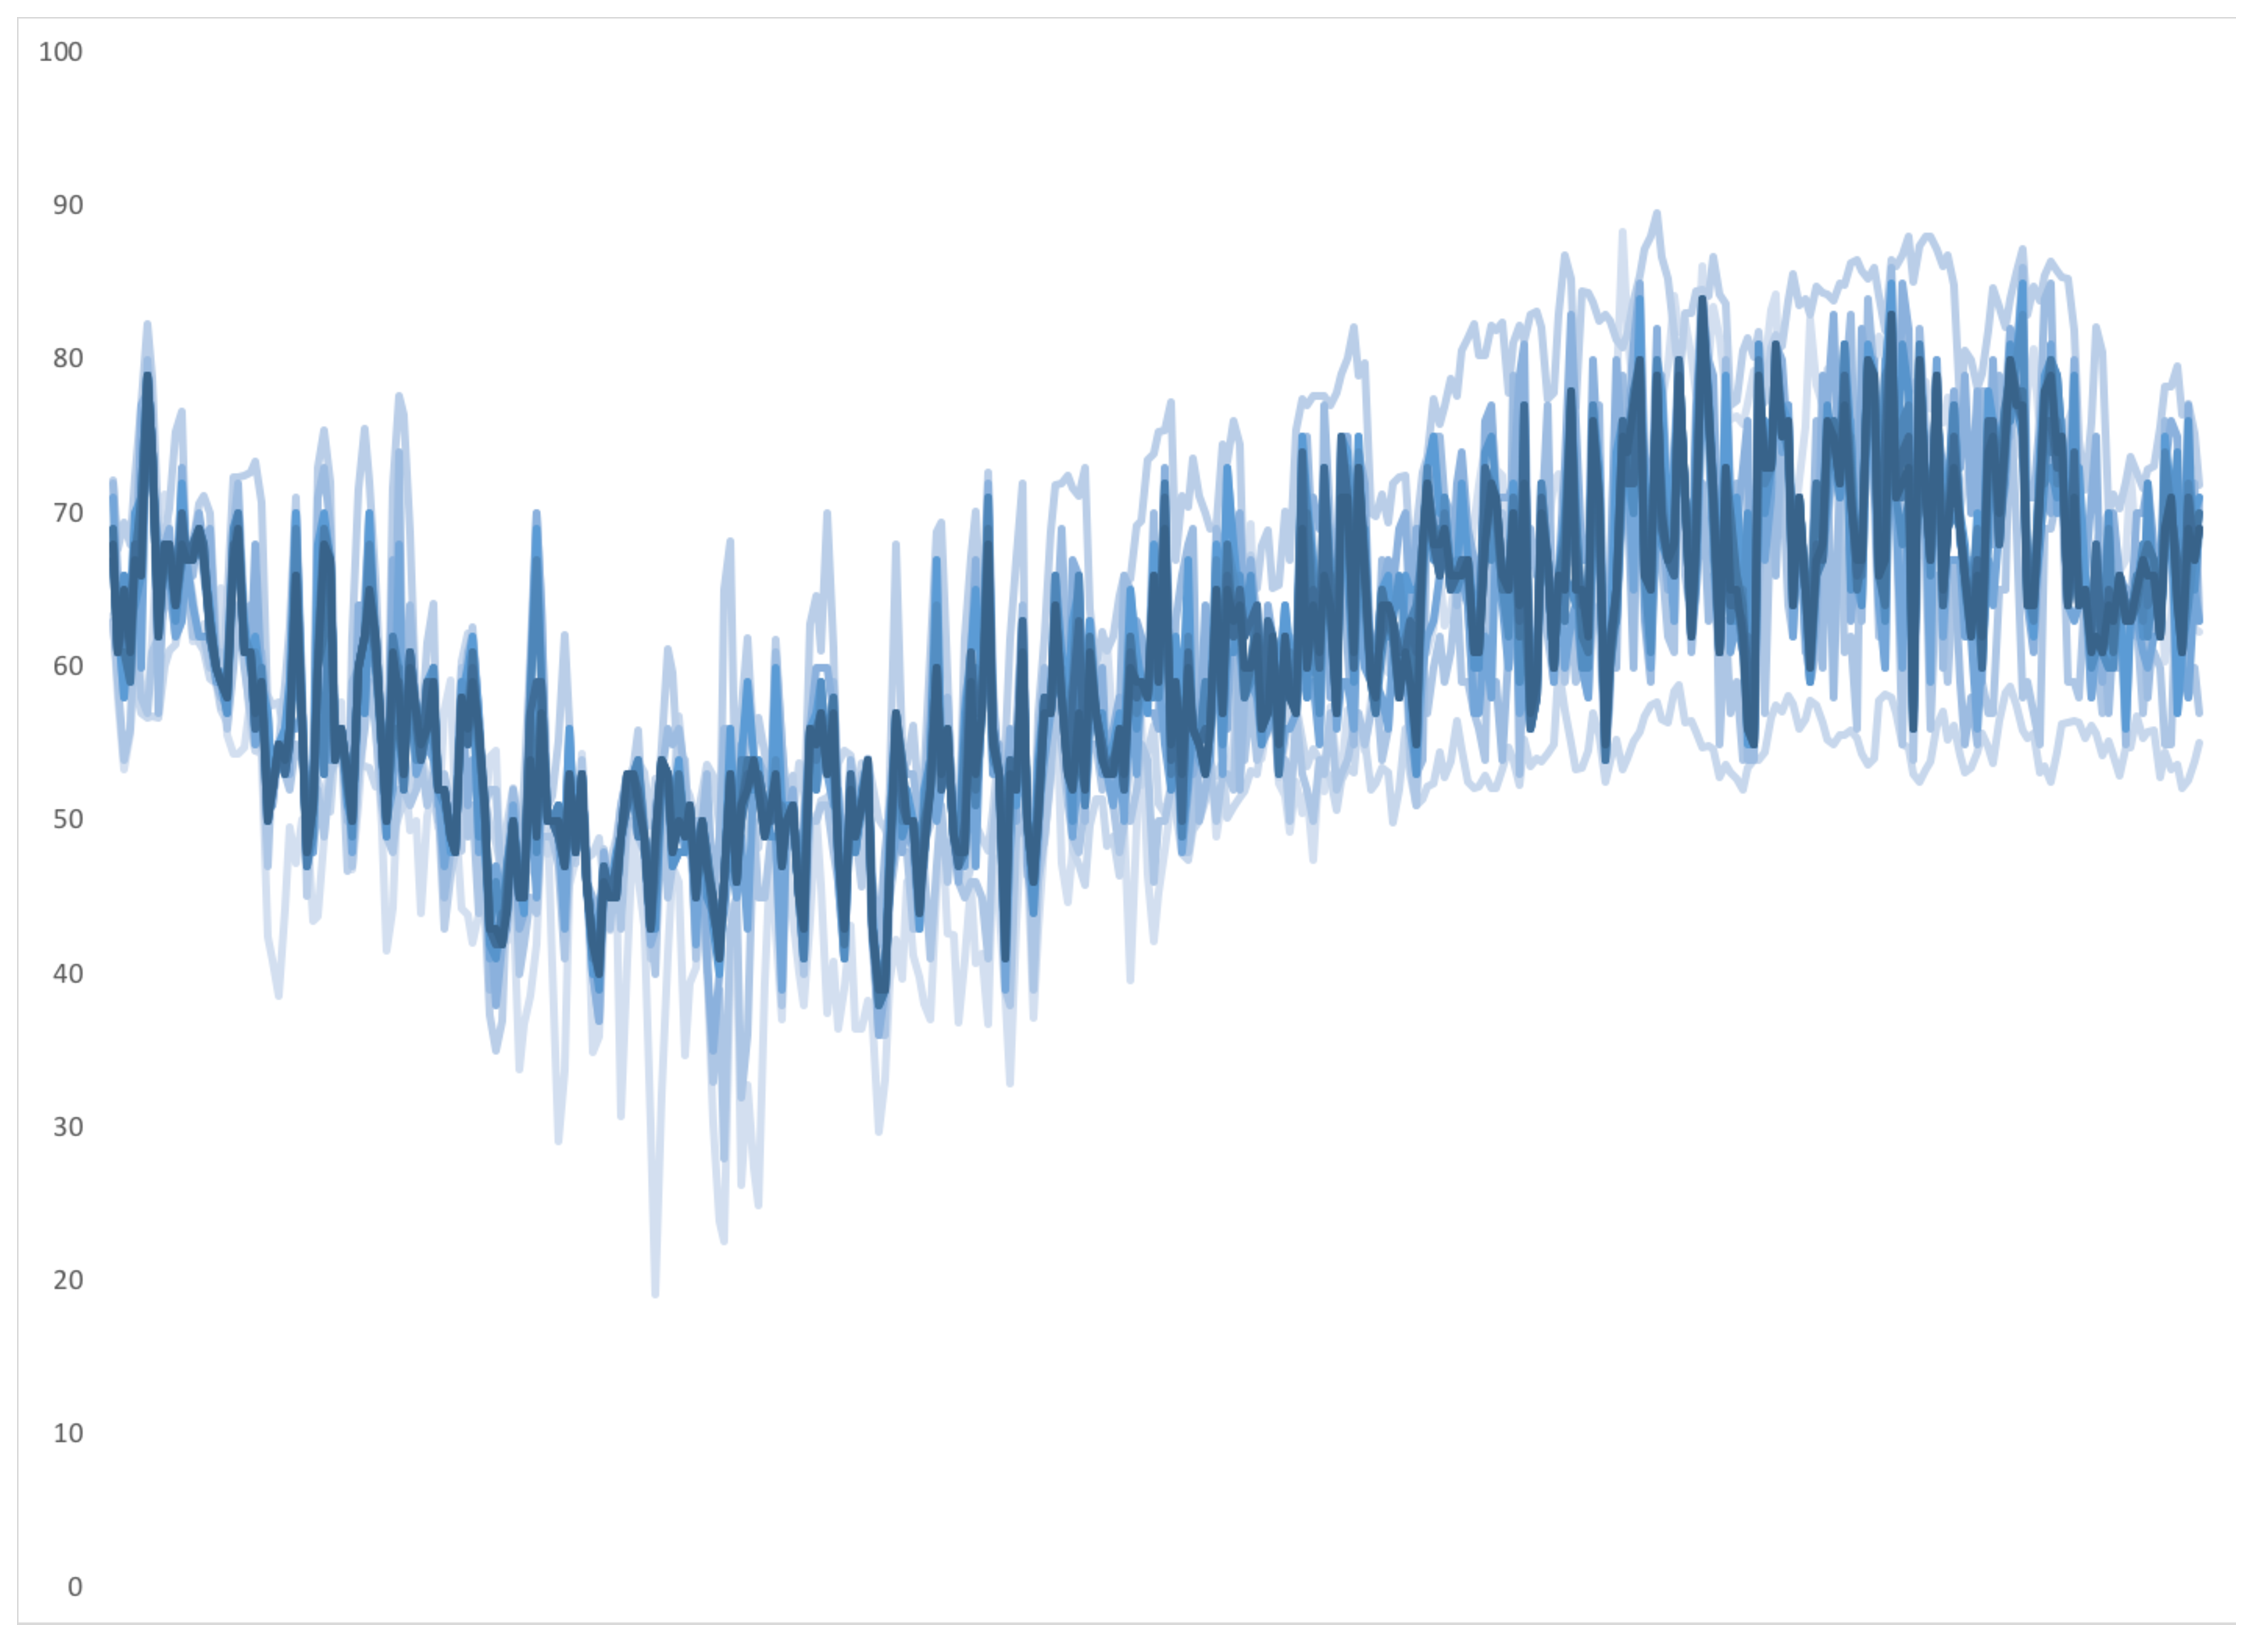
\includegraphics[width=\columnwidth]{images/ensemble}
		\caption{Line ensembles}
	\end{subfigure}%
	~ 
	\begin{subfigure}[t]{.3\columnwidth}
		\centering
		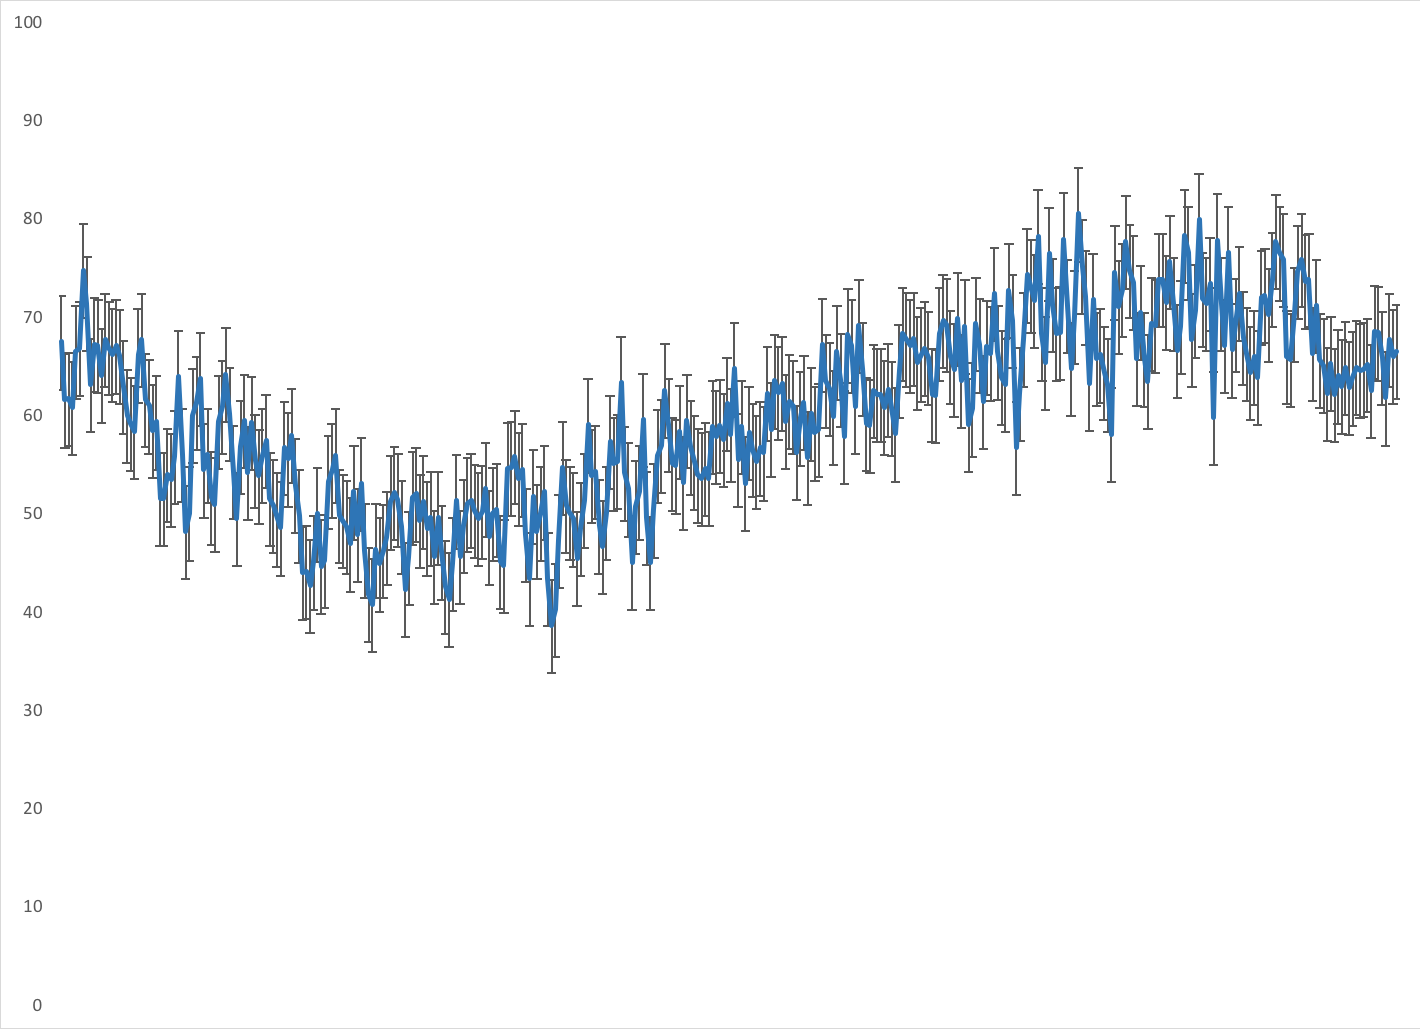
\includegraphics[width=\columnwidth]{images/errorbars}
		\caption{Line with error bars}
	\end{subfigure}
	~ 
	\begin{subfigure}[t]{.3\columnwidth}
		\centering
		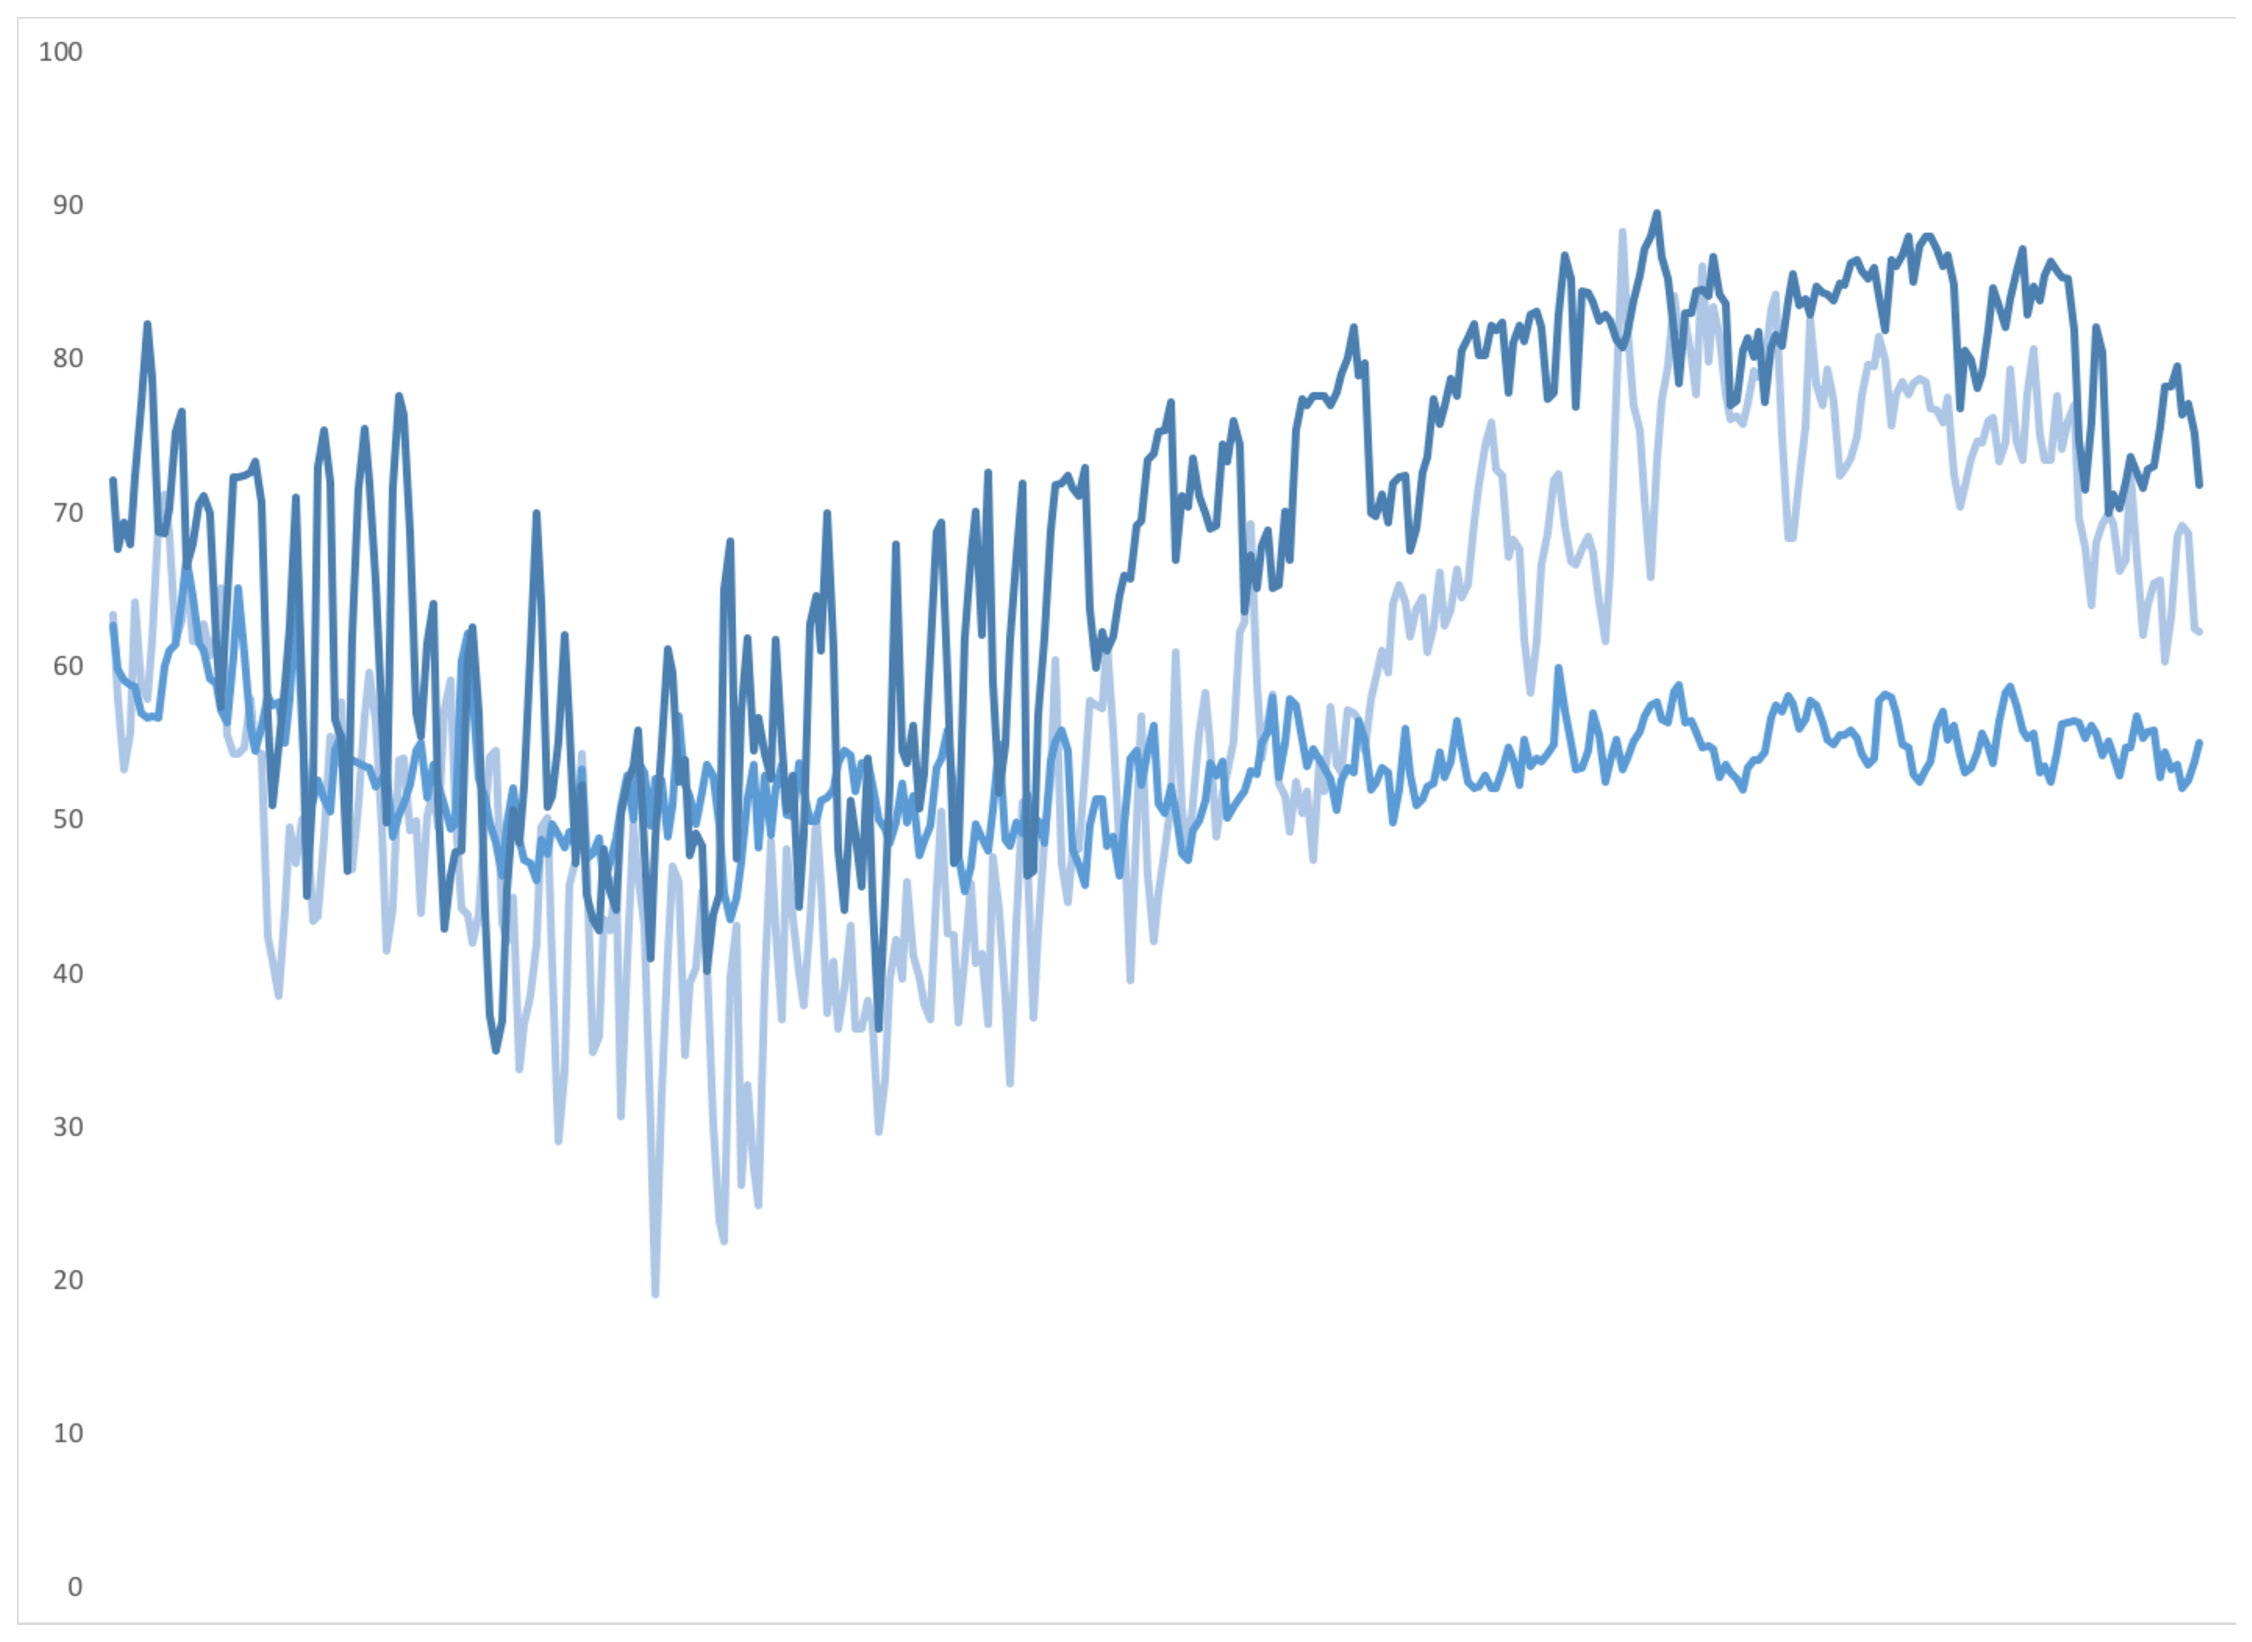
\includegraphics[width=\columnwidth]{images/hops}
		\caption{Hypothetical outcome plots}
	\end{subfigure}
	\caption{We will evaluate visualization techniques for representing uncertainty with time series data. The existed methods include: (a) Line ensembles, (b) error bars, and (c) hypothetical outcome plots~\cite{hullman2015hypothetical}  (an animation that randomly draws from the distribution of possible outcomes.) }
	\label{fig:uncertainty}
\end{figure*}


Communicating uncertainty is one of the greatest challenges we face today.
It impacts many data-driven communities such as climate science~\cite{brodlie2012review,pothkow2011probabilistic,potter2009ensemble,spiegelhalter2011visualizing}, business~\cite{griethe2005visualizing,rodriguez2010toward} and medicine~\cite{han2011varieties,han2011communication,kniss2005statistically,lundstrom2007uncertainty,politi2007communicating,prassni2010uncertainty,spiegelhalter2011visualizing}. 
Visualization has been widely successful in helping people explore, reason, and make judgments with data, and prior work suggests that it may be key for improving comprehension of probability and uncertainty~\cite{correll2014error,brodlie2012review,pothkow2011probabilistic,sanyal2009user,sanyal2010noodles,spiegelhalter2011visualizing}. Researchers have proposed several designs including line ensembles~\cite{potter2009ensemble,sanyal2010noodles}, error bars~\cite{correll2014error}, gradient plots~\cite{correll2014error,han2011communication,jackson2008displaying,tak2014perception} and violin plots~\cite{correll2014error,hintze1998violin,kampstra2008beanplot}. 
More recently, Hullman et al. introduced the hypothetical outcome plot which is an animated chart that randomly draws from the distribution of possible outcomes~\cite{hullman2015hypothetical}. 

One advantage of visualization is that it can make complex or abstract concepts easier to grasp by making them visible. In theory, an effective visual representation can make traditionally difficult problems more concrete and easier to understand. 
In practice, however, nuanced contextual factors heavily impact the effectiveness of visualizations, making the right representation difficult to establish.
While many designs exist, it is not clear whether these methods effective communicate uncertainty and support decision-making in real-world tasks.
Many open questions remain. For instance: \textit{Which visualizations best communicates data with uncertainty}? and \textit{How do
visualizations impact decision-making?}

In this phase of the project, we will explore and evaluate methods for communicating uncertainty to non-experts.
To identify the best techniques, we will rigorously examine existing methods. 
These include using line ensembles (Figure ~\ref{fig:uncertainty}a), using standard error bars (Figure ~\ref{fig:uncertainty}b), using animation (Figure ~\ref{fig:uncertainty}c), as well as other techniques that leverage visual variables (e.g., scaling the size of visual elements, using color to encode the degree of uncertainty, and using transparency or blurring). 
We plan first to test the designs with a diverse population of study participants via Amazon's Mechanical Turk. 
Once we have some candidate visualizations, we will expand these results by testing real aggregated data with clients in their natural work environments.
Dr. Ottley and her team have extensive experience in evaluating systems.
Here we outline the steps we will take to evaluate the different designs.   

\paragraph{Comparing Designs} 
Our goal here is to determine the most effective visualization design for conveying meaningful information and for facilitating decision-making.  
We will conduct experiments via Amazon's Mechanical Turk using three different evaluation approaches.
\begin{itemize}
\item[(1)] We will measure speed and accuracy as participants complete standard search and retrieval tasks.
\item[(2)] Participants will perform decision-making tasks, and we will investigate how each visualization impacts the decisions made.
\item[(3)] During our experiment, we will conduct additional post-tests using adaptations of standard questionnaires. For instance, we will use the NASA-TLX for subjective measures of workload~\cite{hart1988development}, and the System Usability Scale for measuring perceived usability~\cite{bangor2008empirical}. 
\end{itemize}

\paragraph{Client Feedback}
Once we have narrowed the set of prospective visualizations, we will test these candidate designs with real clients. 
We will recruit participants from the BECS annual aquatic sales meeting.   
The clients will interact with the top designs from our previous rounds of experiments. 
For this set of user studies, we will conduct a qualitative evaluation by performing one-on-one observation and collecting clients' feedback.
A typical usability testing of this nature involves techniques such as “think-aloud” exercises, documentation of users’ reported insights, and the time they took to arrive at them~\cite{charlton2001handbook,hix1993developing,lewis1982using}. Findings from this round of testing will also be used to refine the visualization designs.

\paragraph{Application to Visualization Theory} 
Our proposed work of exploring techniques for communicating uncertainty has applications beyond our problem statement. Visualizing uncertainty is a central challenge in the Information Visualization community with many applications including weather, health, business, and government. Evaluating and potentially developing novel visualization techniques for representing uncertainty will be a signification contrition to these application areas.  


\subsubsection{Judging Success}

Ultimately, this project will be successful if we can effectively
protect the privacy of individual data contributors (i.e., a small
privacy budget) concurrently with releasing aggregate data that has
high utility (i.e., low uncertainty).  While theory tells us we cannot
be perfect at one without sacrificing the other, the intention
is to determine how close to that ultimate scenario it is to possible to be.

At the completion of Phase~I, a judgment is required to determine if
further effort towards the above ultimate goal is warranted.
Because that judgment is both a commercial and a technical judgment, we
plan to leverage BECS's annual aquatics sales meeting (which happens in
the fall, typically in November) to help us make that determination.
The sales meeting is timely, in that it happens towards the end of
the Phase~I schedule period.  It is also convenient, in that it is held
in St.~Louis and has attendees who are quite knowledgeable about 
the aquatics industry from around the country (and the world).
Finally, it is inexpensive (at least to the grant), because the full
costs of travel, meeting hall, etc., are all covered by BECS and
the attendees, no STTR funds need be expended.

As described above, during the meeting we will solicit participants
to assist us in evaluating the most promising candidate data visualizations.
In addition, as part of the one-on-one assessment, we will seek their
input as to the levels of privacy that are acceptable and levels of 
uncertainty that are tolerable.
This is how we will judge whether or not we have been successful
in the Phase~I effort.

\subsection{Research Plan}
\label{sec:plan}

The primary participants in the project all reside in St. Louis, Missouri,
so face-to-face meetings have a relatively low overhead. We will coordinate
the project through periodic (e.g., biweekly) meetings that alternate
locations (one meeting at BECS Technology's facility, and two weeks later
another meeting on campus at Washington Univ. in St. Louis).

%Dr. Fan is physically remote (she is in Albany, NY), so her primary
%method of interaction will be via electronic communication.  We will
%use video-conferencing fairly extensively when face-to-face discussions
%are warranted.  In addition, the Dept.~of Computer Science and Engineering
%at Washington University in St.~Louis
%will invite Dr.~Fan to present a colloquium on campus at or very near
%the beginning of the project.  This will enable all of the parties to
%have a true face-to-face interaction without any travel expense charged
%to the grant.

A formal agreement will need to be put in place between the company and
Washington~U.; however, the two organizations have collaborated in the
past (on a previous STTR grant through the National Institutes of Health).
The terms of that previous agreement will form the
basis of the required new agreement, and we anticipate no difficulties
in finalizing the agreement itself.

The proposed research is suited for a twelve-month research agenda.
The schedule is shown in Figure~\ref{fig:gantt}.
The various research components can be independently investigated,
primarily in parallel by the two organizations, coming together
in the assessments to be performed at the sales meeting.

\begin{figure}[h]
 \center
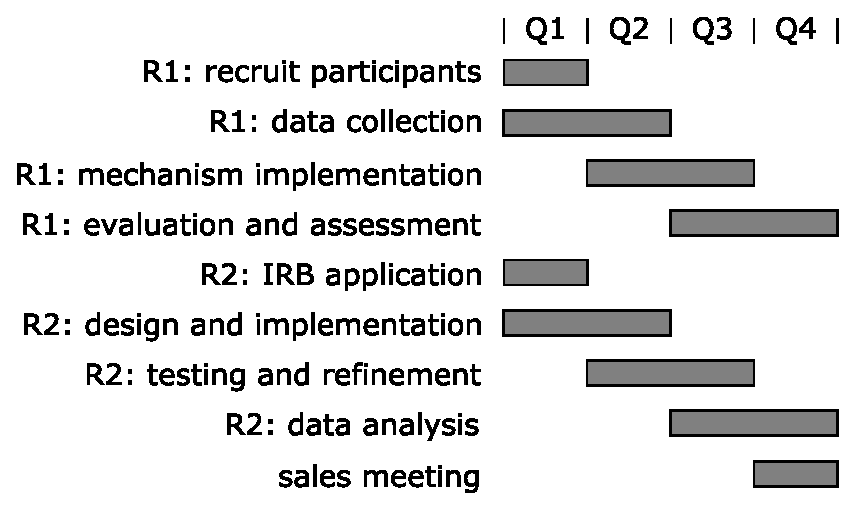
\includegraphics[width=0.5\columnwidth]{gantt}
    \caption{Project schedule, one year duration.}
    \label{fig:gantt}
\end{figure}

The results of the assessments during the sales meeting will inform
the activities to be pursued during Phase~II.
If the result of Phase~I is data that are appropriately anonymized,
one can consider the focus of Phase~II to be the determination of
what it is we can effectively learn from the anonymized data.

The learning from data will come in two forms:
\begin{itemize}
\item {\bf Machine learning} -- we will investigate utilizing techniques
described in the literature~\cite{acgmmtz16,fs10,ss15} for performing machine
learning on differentially private data sets.
We will apply techniques such as these to the problem of water treatment
control, with the goal of diminishing chemical consumption, providing
tighter control, and predicting issues that need human intervention
earlier than they can be detected presently.
\item {\bf Human learning} -- we will explore ways in which we can effectively
communicate to laypersons an intuitive notion of ``privacy budget,'' and
how to visualize risk, which has been studied in the
managment and
financial space~\cite{Eppler09,Sarlin16}, but we are unaware of any
work concerning privacy risk.
\end{itemize}

It is these opportunities for learning that comprise the strongest value
proposition for our customers.  Improved water chemistry, achieved with
greater efficiency, is the true goal of our customers, and this will benefit
primarily from the knowledge gained by aggregating data across organizations,
independent of whether the tranformation from data to knowledge occurs
within BECS (who will share it with customers) or by the customers themselves.

Also, during Phase~II we will investigate the applicability of techniques
we have learned about aquatics data to other domains.  This will start with
agriculture data, as we already have subscription-paying customers in
this market, so the business case could simply be made stronger, rather
than building it from the ground up.
